\documentclass[a4paper]{article}
\usepackage[left=3cm,right=3cm,top=2cm,bottom=2cm]{geometry} % page settings
\usepackage[T1]{fontenc} % use 8-bit font encoding for apostrophes etc.
\usepackage[utf8]{inputenc} % allow foreign characters

\usepackage{graphicx} % embed graphical elements in document

\usepackage{ulem} % underlining

\usepackage{amsmath} % many mathematical environments & tools
\usepackage{amssymb} % mathematical symbols
\usepackage{bm} % bold math symbols

\setlength{\parindent}{0mm} % set indentation for new paragraphs
\setlength{\parskip}{12pt}  % set space between paragraphs

\usepackage{natbib}
% Harvard style
\bibliographystyle{agsm}
% Add the bibliography to the table of contents
\usepackage[numbib,nottoc,notlot,notlof]{tocbibind}

\begin{document}

\title{\LaTeX \, guide}
\author{Jon Lachmann}
\date{\today}
\maketitle

\section{Figures and tables}
We can add figures and tables, and reference them using \verb*|\ref{label}|.

The code below creates table \ref{table:table1} and figure \ref{fig:figure1}.
\begin{verbatim}
	\begin{figure}
		\centering
		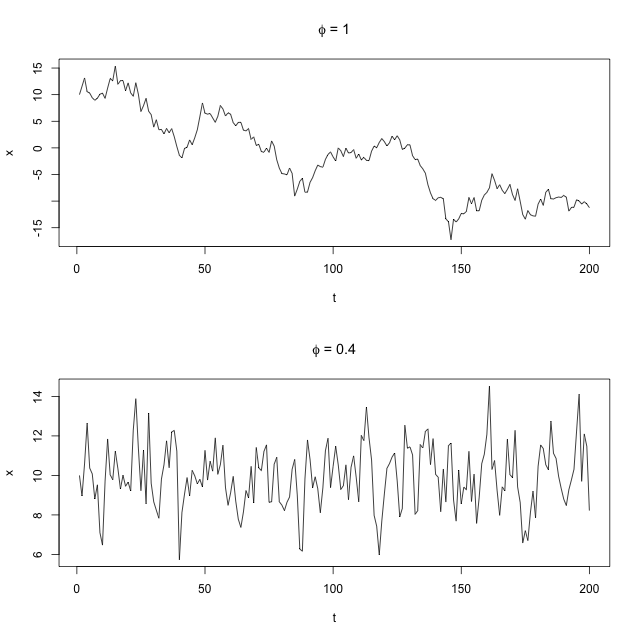
\includegraphics[scale=0.3]{./image}
		\caption{Figure text}
		\label{fig:figure1}
	\end{figure}
	
	\begin{table}[!htbp] \centering
		\caption{Table text} 
		\label{table:table1}
		\vspace{5mm}
		\begin{tabular}{|c|c|}
			\hline
			123&456  \\
			\hline
			789&123  \\
			\hline
		\end{tabular}
	\end{table}
\end{verbatim}

\begin{figure}
	\centering
	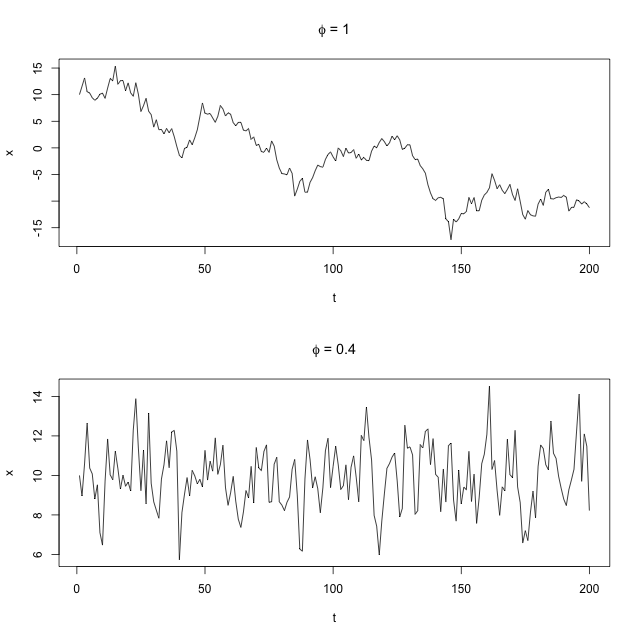
\includegraphics[scale=0.3]{./image}
	\caption{Figure text}
	\label{fig:figure1}
\end{figure}

\begin{table}[!htbp] \centering
	\caption{Table text} 
	\label{table:table1}
	\vspace{5mm}
	\begin{tabular}{|c|c|}
		\hline
		123&456  \\
		\hline
		789&123  \\
		\hline
	\end{tabular}
\end{table}

\newpage
\section{References}
Create a file named \verb*|library.bib| and add "bibtex" blocks to it. These can be found on Google books under "citation" for the book you want to reference. It can also be found on many other sites where material is available. A Google search for any material and "bibtex" usually gives you something.

Put the code below in the header,
\begin{verbatim}
	\usepackage{natbib}
	% Harvard style
	\bibliographystyle{agsm}
	% Add the bibliography to the table of contents
	\usepackage[numbib,nottoc,notlot,notlof]{tocbibind}
\end{verbatim}
and the following line where you want your bibliography in the document, library references the file \verb*|library.bib|
\begin{verbatim}
	\bibliography{library}
\end{verbatim}

Make an inline reference using \verb*|\citet{bookid}|, and one in parentheses using \verb*|\citep{bookid}|.

As was mentioned in \citet{wonnacott1979econometrics}, bla bla bla...

Econometrics is a subject \citep{wonnacott1979econometrics}.

\bibliography{library}







































\end{document}
